\chapter{Bitcoin Transactions and Scripts}

Before Bitcoin in the late 90s there was an idea for a digital currency called \texttt{e-Cash}.
\texttt{e-Cash} introduced the concept of \textbf{blind signatures}, which allowed a bank to sign a transaction without knowing the details of the transaction.
The concept was to go a step further than plain public key cryptography, by adding a \textbf{nonce}\footnote{Random number} to be ---mathematically--- combined with the data in transit, obtaining \textit{``scrambled data''}.
The bank would \textit{``blind sign''} the scrambled data, without being able to know the original data.

\section{Bitcoin release}

{Later on, in 2008, Satoshi Nakamoto\footnote{This is a pseudonym, the actual name of the author is unknown} introduced Bitcoin, a decentralized digital currency, with some key properties:\ns
\begin{itemize}
   \item \textit{Double-spending} is prevented with a peer-to-peer network.
   \item No mint or other trusted parties.
   \item Participants can be \textit{anonymous}.
   \item New coins are made from Hashcash style \textit{proof-of-work}.
   \item The \textit{proof-of-work} for new coin generation also powers the network to prevent \textit{double-spending}
\end{itemize}}

Bitcoin differs from \texttt{e-Cash} in that it is a decentralized and \textit{unstructured} entirely P2P system, with no central authority such as banks.

\subsection{Unhappy episodes}
In 2014 Mt GOX, a Bitcoin exchange, filed for bankruptcy after losing 850,000 Bitcoins, worth \$473 million at the time; they were most likely stolen, probably due to a vulnerability in the protocol (\textit{malleability} will be discussed later on).

Up to 2013, the Silk Road was an online black market, best known as a platform for selling illegal drugs. It was shut down by the FBI in 2013, and the founder, Ross Ulbricht, was sentenced to life in prison.

Even now, ransomware attackers demand payment in Bitcoin, as it is difficult to trace and provides pseudo anonymity through the use of Bitcoin addresses.

\section{Bitcoin Identity}
An easy way to generate new identities in a cryptographic system is to create a new random key-pair, made up of a private ---secret--- key \texttt{sk} and a public key \texttt{pk}, which acts as the ``public name'' of an user.
In case  \texttt{verify(pk, data, sig) == true} then the transaction signed with \texttt{sig} was generated by \texttt{pk}. 

\begin{figure}[htbp]
   \centering
   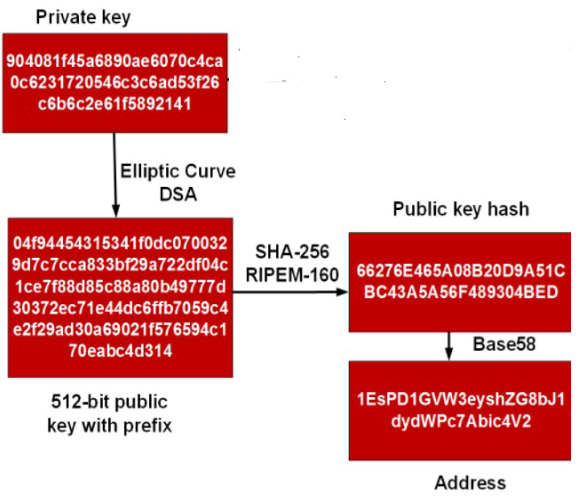
\includegraphics{images/bitcoin_addressgen.png}
   \caption{Bitcoin address generation process}
   \note{
      \texttt{Base58} is used to eliminate from the 62 alphanumerical alphabet the characters \texttt{(0,O,l,I)} which may appear identical when displayed in certain fonts.
   }
   \label{fig:bitcoin_addressgen}
\end{figure}

Addresses in the majority of cases represent the owner of a private/public key pair, and are generated using \texttt{pk}, but they may also be a \textbf{script}.

Anyone can make a new identity at any time, and such identities are not necessarily linked to any real-world identity, but the activity of an identity may be observed over time ---the blockchain is in clear readable by anyone--- and thus make inferences on to whom it may belong.

\section{Bitcoin Transactions}

\begin{figure}[htbp]
   \centering
   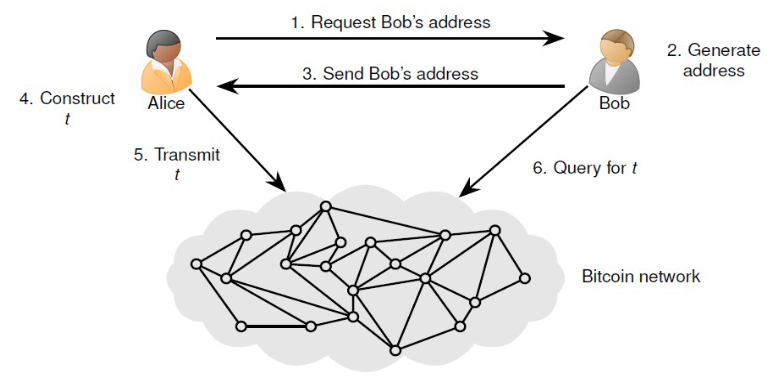
\includegraphics{images/bitcoin_workflow.png}
   \caption{Bitcoin transaction workflow}
   \note{Note that the address exchange is performed out-of-band, not through the Bitcoin P2P network}
   \label{fig:bitcoin_workflow}
\end{figure}

A transaction \textit{t} is used to transfer funds from the sender to the receiver, and is registered on the blockchain when confirmed.
The transaction \textit{t} is broadcasted to the network; miners collect broadcasted transactions and include them in a candidate block.
When a miner solves the Proof of Work, the block is broadcasted to the network, and ---if the block includes $t$--- the transaction $t$ is confirmed.

\begin{figure}[htbp]
   \centering
   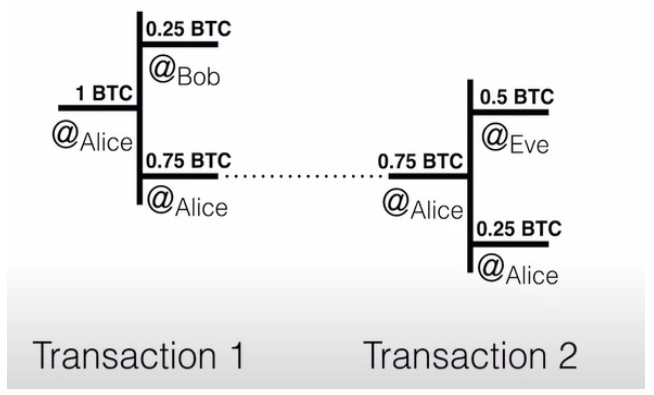
\includegraphics{images/bitcoin_transaction.png}
   \caption{Bitcoin linked transactions}
   \label{fig:bitcoin_transaction}
\end{figure}

On the left of each transaction there is a list of inputs, and on the right a list of outputs. 

Consider Fig. \ref{fig:bitcoin_transaction}: in the left transaction, 0.25 is the money requested by Bob, 1.00 is the money given by Alive and 0.75 is the change she gets back.\\
Every input must equal the outputs, but note that this should include a \textbf{transaction fee}, computed as the difference between the inputs and the outputs, and is given to the miner who confirms the transaction.

It is possible to \textbf{merge} or \textbf{distribute}, in the first case, multiple inputs are used to create a single output, in the second case, a single input is used to create multiple outputs.
So, as said, transactions may also be \textbf{multi input} as depicted in Fig. \ref{fig:bitcoin_multiinput}.

\begin{figure}[htbp]
   \centering
   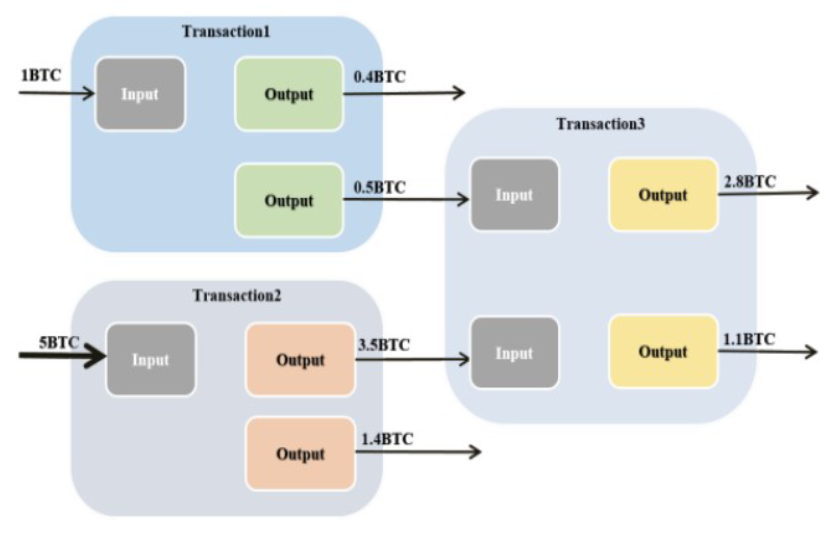
\includegraphics{images/bitcoin_multiinput.png}
   \caption{Multi input transaction}
   \label{fig:bitcoin_multiinput}
\end{figure}

\subsection{UTXO Model vs Bank Accounts}
Typical centralized currencies exploit ``bank'' accounts and \textit{transfers} between to move the money from one account (``person'') to another.
Also Ethereum follows this approach, while Bitcoin adopted the UTXO one, which is based on \textbf{unsent output addresses}, i.e. addresses containing bitcoins and not spent in any
transaction.

\begin{definition}[UTXO]
   \label{def:UTXO}
   A UTXO represents a certain amount of cryptocurrency that has been authorized by a sender and is available to be spent by a recipient.
   UTXOs employ public key cryptography to ascertain and transfer ownership. More specifically, the recipient's public key is formatted into the UTXO, thereby limiting the capability to spend the UTXO to the account that can demonstrate ownership of the corresponding private key. A valid digital signature associated with the public key must be included for the UTXO to be spent.\\
   \href{https://en.wikipedia.org/wiki/Unspent_transaction_output}{Wikipedia}
\end{definition}

Each transaction input is linked (refers) an UTXO of
a previous transaction, while each output generates a new UTXO, which is included in the user's wallet and is available to be spent.
Each UTXO is \textit{spent} (thus is no more an UTXO) if it is linked to the input of a subsequent transaction.\\
Getting the the \textbf{balance} of an address, equals to scanning the network for UTXOs and adding up all the unspent output locked to that address.

\begin{figure}[htbp]
   \centering
   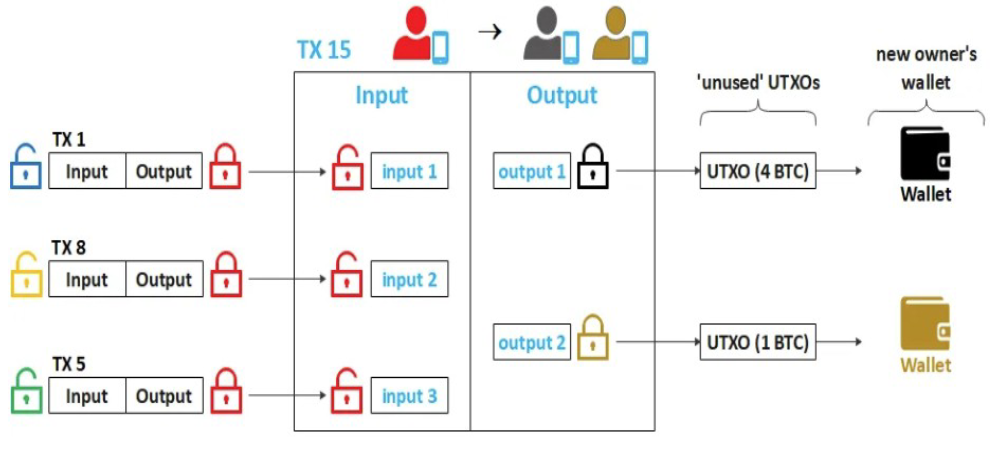
\includegraphics{images/bitcoin_UTXO.png}
   \caption{UTXO locking}

   Each UTXO \textit{``locks''} the newly generated UTXO to the new owner's public key, and if they decide to use the UTXO in a new transaction, it must \textit{``unlock''} the funds with their private key.
   \label{fig:bitcoin_UTXO}
\end{figure}

\begin{figure}[htbp]
   \centering
   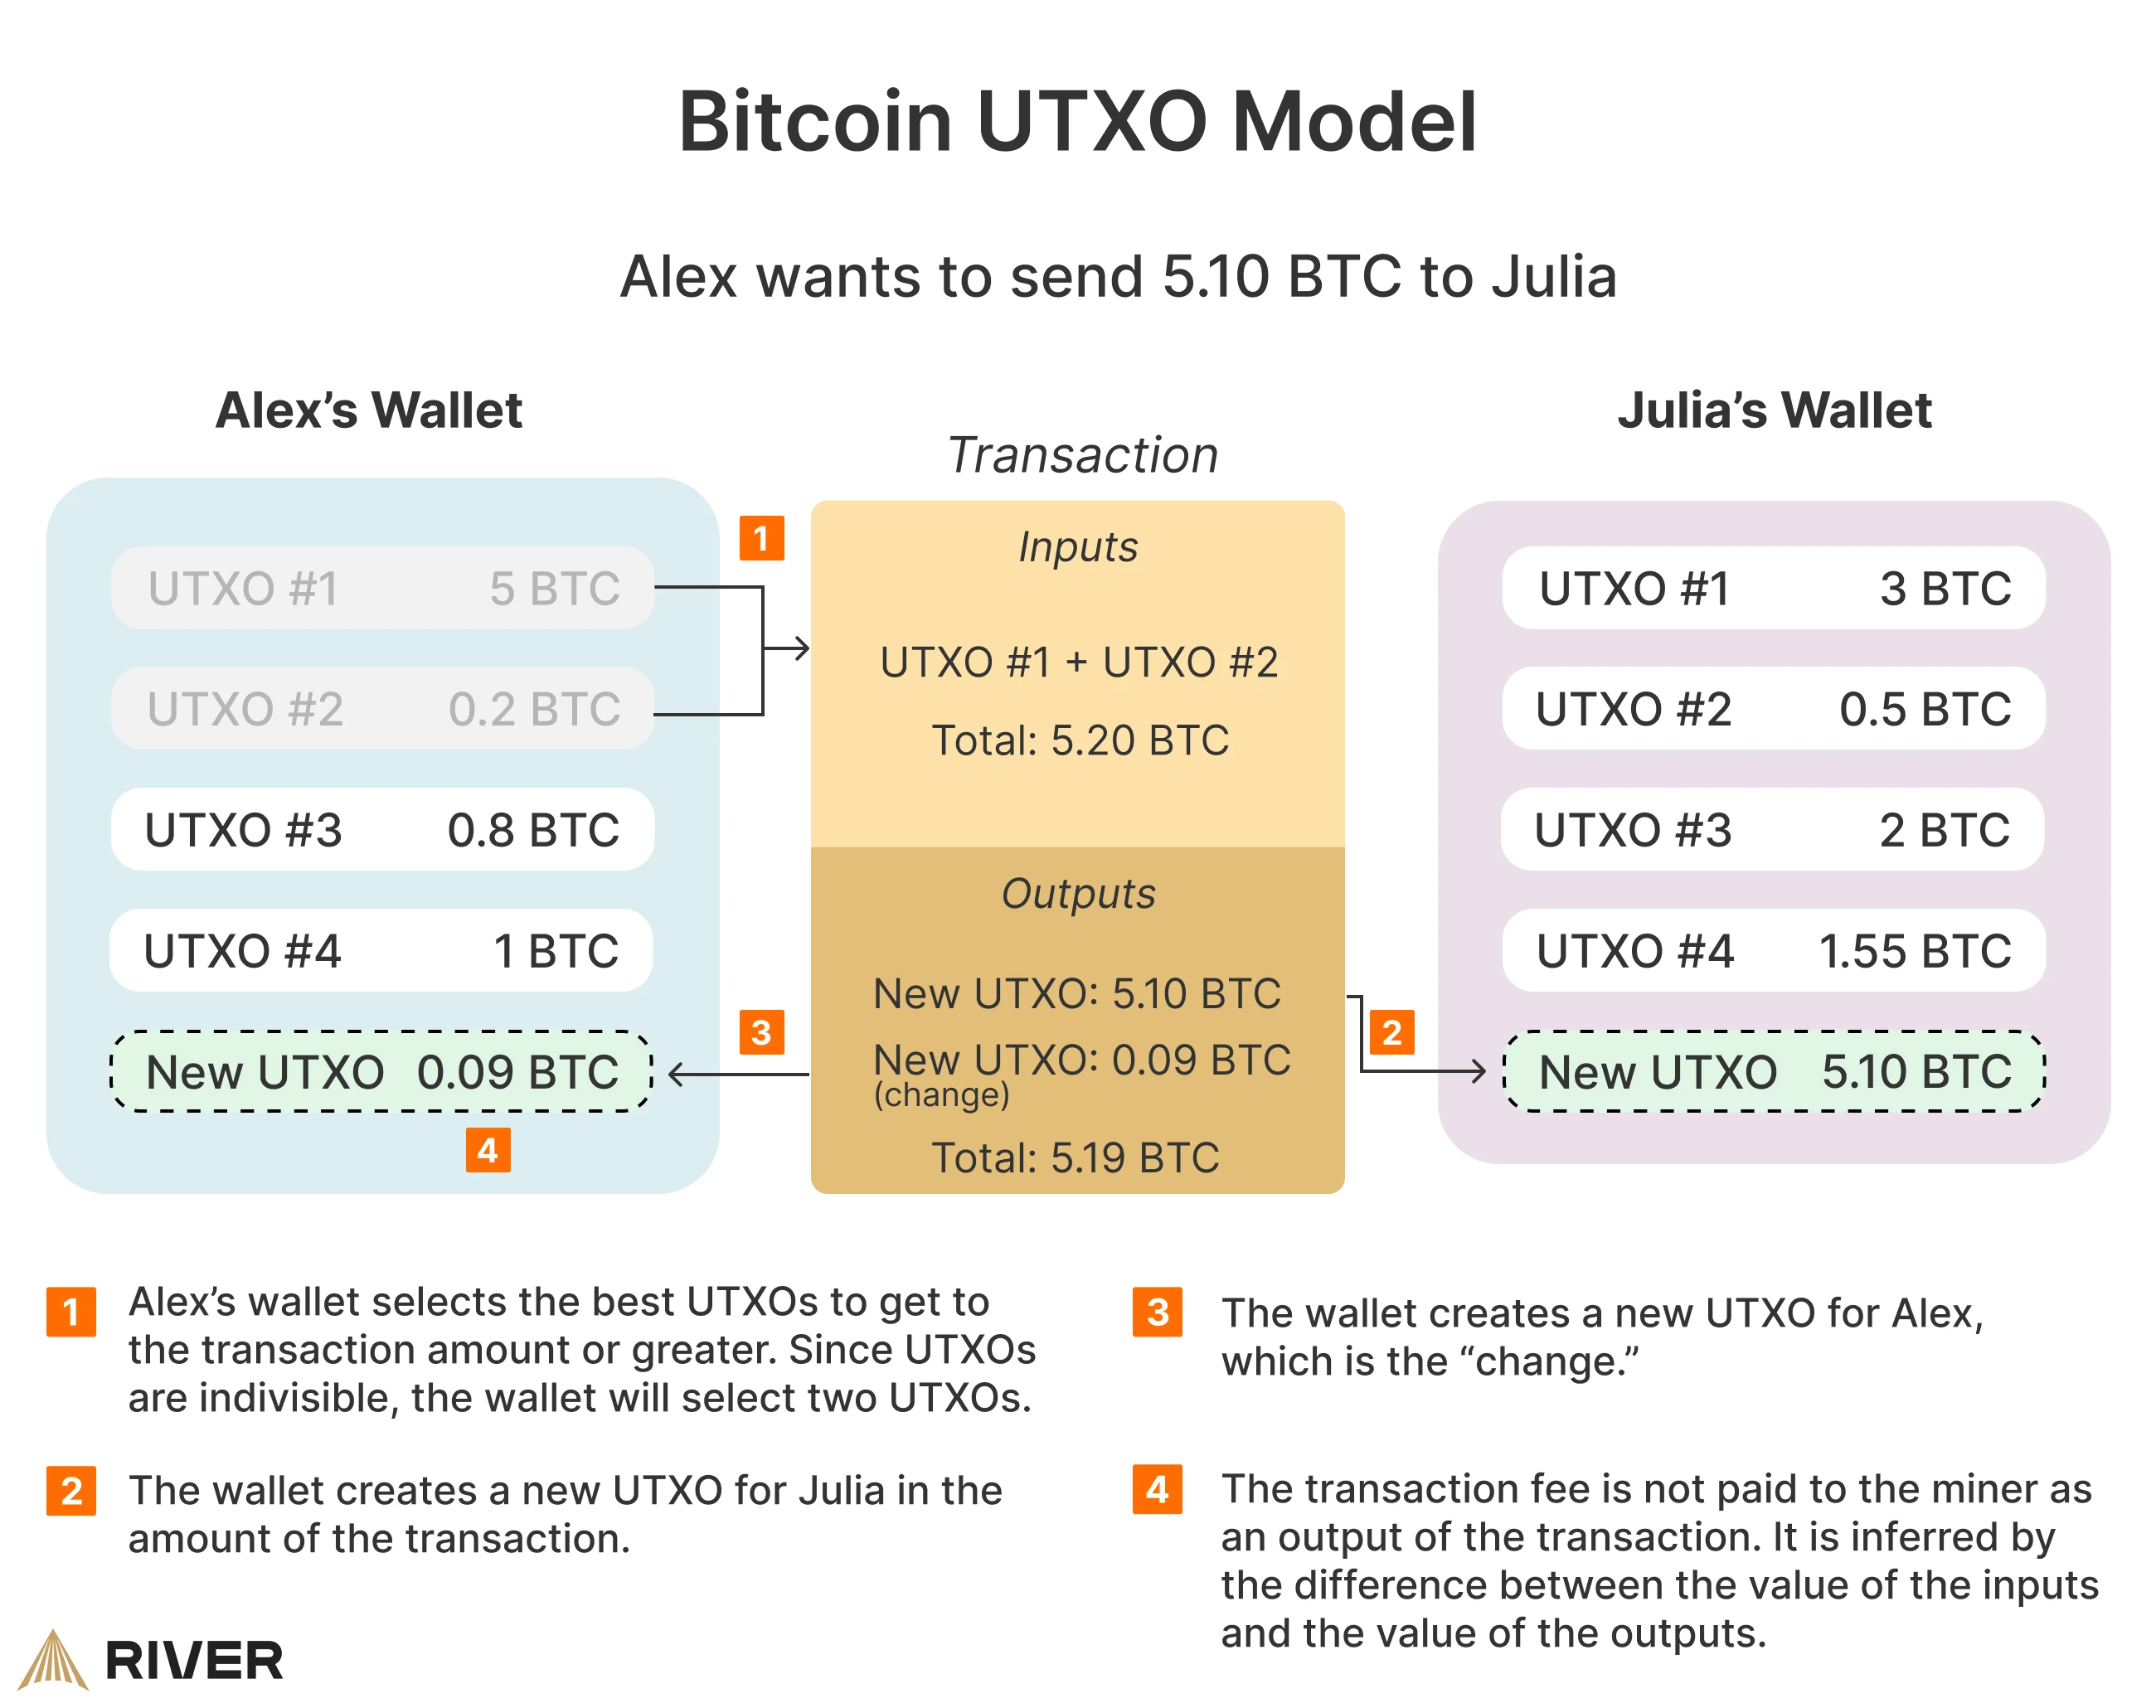
\includegraphics{images/bitcoin_utxo_model.png}
   \caption{More comprehensive example explaining how UTXOs are related to transactions}
   \label{fig:bitcoin_utxo_model}
\end{figure}


\newpage
\subsection{Scripts}
\begin{figure}[htbp]
   \centering
   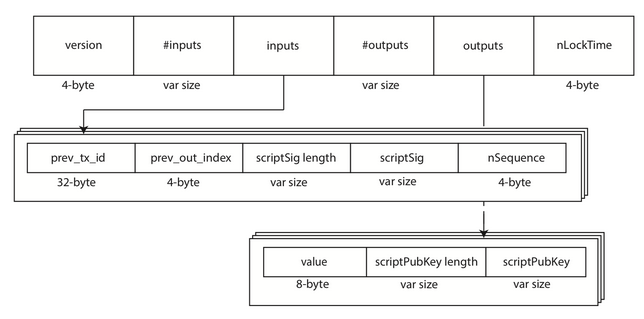
\includegraphics{images/bitcoin_transactionStructure.png}
   \caption{Bitcoin Transaction structure}
   \label{fig:bitcoin_transactionStructure}
\end{figure}

Each transaction contains a \textbf{script} written in a simple and ---intentionally--- limited language\footnote{Not Turing-complete and overall limited to avoid endless looping and execution errors.} to check the ownership of the transferred funds.\\
Script execution is stateless and completely deterministic.
Typical use case is signature verification.
Script types include:
\begin{itemize}
   \item Pay to Public Key (P2PK)
   \note{Most simple case}
   \item Pay to Public Key Hash (P2PKH)
   \note{Most common case}
   \item Pay to Script Hash (P2SH)
   \item Pay to Multi-signature
\end{itemize}

\subsubsection{Simplified locking and unlocking}
\begin{figure}[htbp]
   \centering
   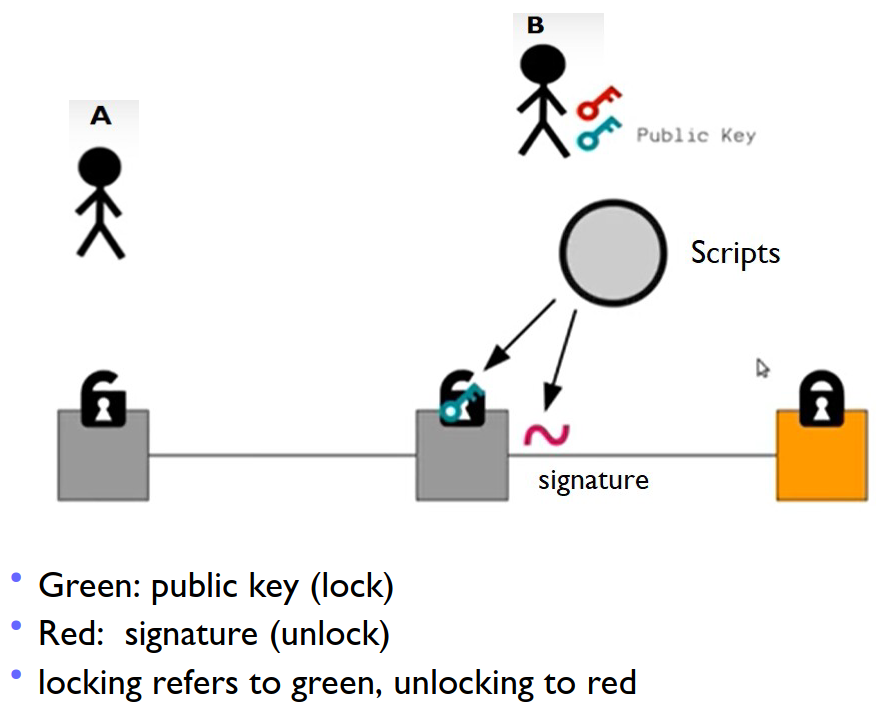
\includegraphics{images/bitcoin_script.png}
   \caption{Bitcoin script example}
   \label{fig:bitcoin_script}
\end{figure}
\framedt{Put simply}{
   B first notifies its public key to A, who now knows to whom to send the bitcoin.
   A unlocks some of its bitcoins ---locked by a previous transaction--- and creates a lock on the bitcoin sent to B, which can be unlocked by B using its private key.
}

But what actually happens is this:
\begin{enumerate}
   \item \textit{Alice} chooses the UTXO\footnote{Or more UTXOs from multiple transaction} of a transaction $t_1$ from \textit{Eve} to her. Inside $t_1$ there is a script that locks the UTXO to \textit{Alice}'s public key.
   \item \textit{Alice} creates a new transaction $t_2$ to send some bitcoin to \textit{Bob}. $t_1$ is indicated as input for $t_2$. $t_2$ includes a script which unlocks the funds from $t_1$ and locks and a locking script which binds the output of $t_2$ to \textit{Bob}'s public key.
   \item Nodes will verify ---among other things--- that \lstinline{eval(t1.locking_script | t2.unlocking_script)} is true.
\end{enumerate}

\subsubsection{Analyzing P2PKH}
As stated before, the outline of a transaction is as follows:\\
The sender appends a script onto sent bitcoin to lock the transferred bitcoin (the UTXO should include the locking script) and make it usable only by the receiver, which is the only one able to write a script (signature) to unlock the bitcoin.
The unlocking script is prepended to the locking script retrieved from the input UTXO, and the result is executed by the Bitcoin network to verify that the sender can actually spend the funds.\\
The transaction output includes the locking script, which will be used by the recipient when spending the funds.
Executing both unlocking and locking scripts allows the receiver to spend the bitcoin.

In the case of P2PKH, the locking script is a \texttt{Pay to Public Key Hash} script, which is a script that locks the UTXO to the public key hash of the receiver, i.e. the address.
In the default case, the unlocking script is a signature of \textit{all} input and output fields of the transaction, but it's not necessarily like that (See \ref{sec:bitcoin_signatures}).
\begin{paracol}{2}

   Execution is stack based, so first \texttt{Sig} and \texttt{PubK} are pushed on the stack, then the \texttt{OP\_DUP} duplicates the top element of the stack, \texttt{OP\_HASH160} hashes the top element of the stack, \texttt{OP\_EQUALVERIFY} checks if the top two elements are equal, which are the newly generated hash and the \texttt{PubKHash} contained in the locking script,
   lastly \texttt{OP\_CHECKSIG} expects \texttt{Sig} and \texttt{PubK} to be in the stack and verifies the \textit{signature}.
   The signature may have been performed an all output fields of the transaction, or only to a single one, or none. (See below \ref{sec:bitcoin_signatures} for more)
   
   \switchcolumn
   \colfill
   \begin{figure}[htbp]
      \centering
      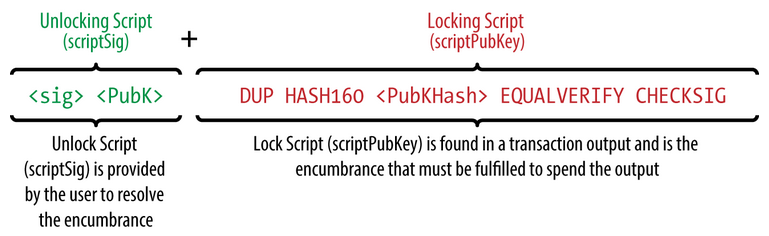
\includegraphics[width=0.95\columnwidth]{images/bitcoin_p2pkh.png}
      \caption{Pay to Public Key Hash}
      Here \texttt{PubKHash} is the hash of the public key of the receiver.
      \label{fig:bitcoin_p2pkh}
   \end{figure}
   \colfill
   
\end{paracol}

\framedt{Signature types}{
   \label{sec:bitcoin_signatures}
   \begin{itemize}
      \item \texttt{SIGHASH\_ALL} signs all the output fields (default)
      \item \texttt{SIGHASH\_SINGLE} signs only the output field corresponding to the ``current input index''
      \note{\textit{``sign \textbf{one} of the outputs-- I don't care where the other outputs go.''}}
      \item \texttt{SIGHASH\_NONE} signs none of the output fields
      \note{\textit{``sign \textbf{none} of the outputs-- I don't care where the bitcoins go''}}
      \item \texttt{SIGHASH\_ANYONECANPAY} signs only the current \textit{input} (This may be applied after one of the other three)
      \note{\textit{``Let other people add inputs to this transaction, I don't care where the rest of the bitcoins come from.''}}
   \end{itemize}

   \note{See \href{https://en.bitcoin.it/wiki/OP_CHECKSIG}{en.bitcoin.it/wiki/OP\_CHECKSIG} for more info}

}

\note{To better understand how locking works, check out \href{https://bitcoin.stackexchange.com/questions/75165/what-is-bitcoin-locking-and-unlocking-script}{this stackexchange discussion}. It provides a fairly detailed description of the process.\\
It might be helpful to give a look also at \href{https://learn.saylor.org/mod/book/view.php?id=36364&chapterid=18948}{this brief page on the topic.}}
\subsubsection{Coinbase Transaction}
Coinbase transactions involve fresh bitcoins generated by the system used to reward miners for solving the Proof of Work, and are not linked to any previous transaction.

\subsection{Transaction Lifecycle}
\labelitemize{Lifecycle}{
   \begin{enumerate}
      \item Starts with the transaction's \textbf{creation}
      \item Then the transaction is \textbf{signed} with one or more signatures indicating the
      authorization to spend the funds referenced by the transaction. 
      \note{(See digression on signatures types \ref{sec:bitcoin_signatures})}
      \item It is \textbf{broadcasted} on the Bitcoin P2P network
      \item Each network node (participant) validates and \textbf{propagates} the transaction
      until it reaches (almost) every node in the network.
      \item The transaction is verified by a mining node and included in a \textbf{block} of
      transactions recorded on the blockchain.
      \item Once recorded on the blockchain and \textbf{confirmed} by sufficient subsequent
      blocks (confirmations), the transaction is a permanent part of the blockchain
      \item The funds allocated to a new owner by the transaction can then be \textbf{spent} in a
      new transaction, extending the chain of ownership
   \end{enumerate}
}